% this file is called up by thesis.tex
% content in this file will be fed into the main document

%: ----------------------- name of chapter  -------------------------
\chapter{Proposed Methods} \label{ch4}% top level followed by section, subsection

In Chapter \ref{ch3}, we recognized three essential gaps in the related work. Firstly, the potential of using new machine learning algorithms that handle categorical variables, specifically  \textit{CatBoost}, to predict the outcome in the context of business processes has not been explored. Then, Exploring different sequence encoding methods to obtain a lossless encoding of the feature vector, in particular, \textit{Discrete Wavelet Transformation.} Finally, studying the potential of using \textit{inter-case} features since in real-life systems the outcome does not depend on the running case only, but it depends on features that come from the concurrent execution of all business cases. 

This Chapter will clarify the subsequent research questions:


\begin{itemize}[itemindent=0em]
	\item[\textbf{RQ4}] How to improve the current outcome-oriented predictive process monitoring approaches in terms of performance?	
\end{itemize}

To answer RQ4, we propose solutions to the mentioned three gaps, starting with CatBoost in section \ref{catb}, followed by wavelet transformation in section \ref{dwt}, and ending with inter-case features in section \ref{inter}.


%: ----------------------- paths to graphics ------------------------

% change according to folder and file names
\ifpdf
    \graphicspath{{X/figures/PNG/}{X/figures/PDF/}{X/figures/}}
\else
    \graphicspath{{X/figures/EPS/}{X/figures/}}
\fi

%: ----------------------- Mobile Cloud Middleware ------------------------

\section{CatBoost} \label{catb}
\textit{CatBoost} is one of the most potent and recent gradient boosting (i.e. a type of machine learning algorithms that work very well with heterogeneous data, i.e. does not have a specific internal structure, that is based on decision trees) algorithms. Motivation to use CatBoost in outcome-oriented PPM comes from the great results that are shown on a variety of publicly available datasets. CatBoost is very stable to parameter changes \cite{prokhorenkova2018catboost} which means using it with default parameters often wins all other methods with tuned parameters. 

\textbf{Cat}boost (i.e. Categorical Boosting) differs from other gradient methods through three main things: (\romannumeral 1) Way to build trees; (\romannumeral 2) Categorical features handling; (\romannumeral 3)  Boosting method; We will compare CatBoost algorithm with other gradient methods (see figure \ref{fig:catb}) such as XGBoost (i.e. Extreme Gradient Boosting), and LGBM (i.e. Light Gradient Boosting Machine) to show why we introduce this method into outcome-oriented predictive process monitoring.


\begin{figure}[htb]
	\begin{center}
		\resizebox{10cm}{!}{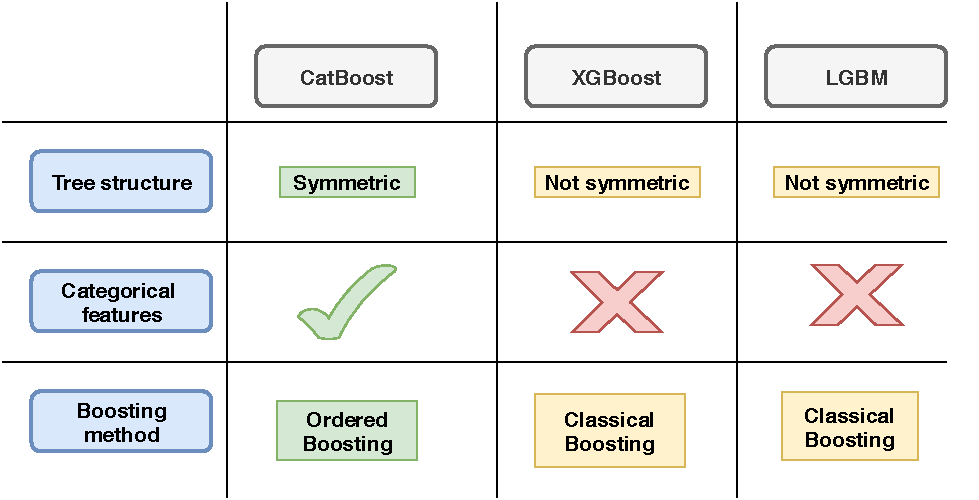
\includegraphics{images/general/catb.pdf}}
		\caption[CatBoost vs XGBoost vs LGBM]{A comparison between gradient boost methods, i.e. CatBoost, XGBoost, and LGBM w.r.t., the way each method used to construct trees, tackling categorical features, and boosting method. }
		\label{fig:catb}
	\end{center}
\end{figure}

\textit{Tree structure}. LGBM builds trees in a greedy fashion node by node and using this way; we can get a very deep, not symmetric tree \cite{ke2017lightgbm}. XGBoost builds trees layer by layer and then prunes them, which means it does not go deeper, and the resulting trees are not symmetric that lead to over-fitting. CatBoost uses full binary trees that are symmetric. This type of tree gives more simple predictors which means the algorithm is less go into over-fitting, and it also helps the algorithm to be more reliable to parameter changes.

\textit{Categorical handling.} For categorical features, current algorithms either do not work with them at all such as XGBoost or deal with them in a not optimal way like LGBM, and the most common method to tackle categorical features is to use one-hot encoding. CatBoost handles categorical features in a very efficient way. It does a set of things w.r.t categorical features: (\romannumeral 1) The first and most important thing in terms of quality is \textit{statistics based on category and category plus label value.} In this step, it calculates a new set of numerical features based on the current existing categorical ones. Numerical features are calculated based on statistics related to category, e.g. the number of appearances of categories and at the same time based on label value, e.g. the average label value among objects that have the same category. For a binary classification it is the probability of having success in the given category for example (see figure \ref{fig:cat1}) the new numerical feature value based on those statistics for object $i$ is $P(1 \mid A) = \frac{3}{4}$, but this method leads to over-fitting. One way to overcome this problem, for each object, e.g. $i$ averages are calculated differently in particular, for object number $i$ objects that are before it is used to calculate average statistics and label of object $i$ is never used during the calculation. For example, the object $i$ has three objects before the given one at index $4$, and the generated numerical feature is equal to $\frac{2}{3}$.  If an object is the first one in the data set when we have zero by zero, then the \textit{prior} value is needed, and for each feature, different priors are selected internally to make better qualities \cite{prokhorenkova2018catboost}; (\romannumeral 2) Usage of several permutations to choose tree structure; (\romannumeral 3) Greedy constructed feature combinations, i.e. combine categorical features, e.g. \textit{colour and animal} features become after combining them \textit{blue\_cat, or red\_dog} and in many cases these combinations are meaningful; (\romannumeral 4) One hot encoding that works well if the data set has a small number of categories, e.g. gender (male or female).

\begin{figure}[htb]
	\begin{center}
		\resizebox{10cm}{!}{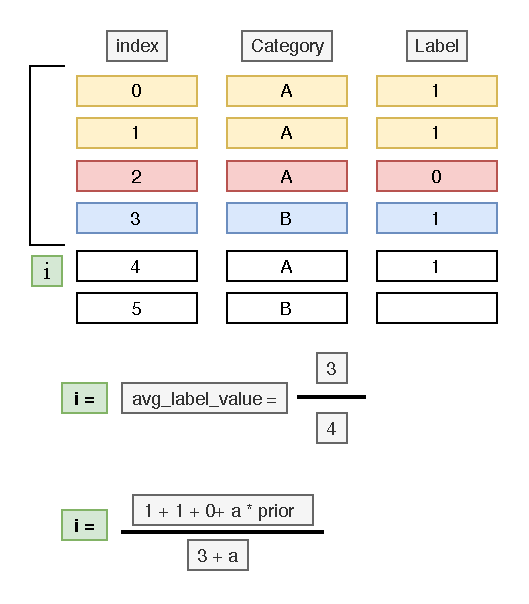
\includegraphics{images/general/cat1.pdf}}
		\caption[Categorical handling in CatBoost]{CatBoost tackles categorical features by calculating some statistics on the basis of the current and previous objects.}
		\label{fig:cat1}
	\end{center}
\end{figure}


\textit{Boosting method}. In most gradient methods such as XGBoost and LGBM, they use \textit{classical boosting} where leaf values (see equation \ref{eq1}) are calculated based on the average of all gradients in the leaf. This method is prone to over-fitting since all gradient estimates are always biased. CatBoost uses \textit{ordered boosting} where gradient estimate is done for objects separately using a separate model, and accordingly, the estimate is unbiased (see equation \ref{eq2}). This method is \textit{quadratic} per each iteration for memory and time, so instead of training $n$ different models, we train $log(n)$ models \cite{prokhorenkova2018catboost}.


\begin{equation} \label{eq1}
\begin{split}
leafValue & = \sum_{i}^{n} \frac{g(approx(i), target(i)}{n}   
\end{split}
\end{equation}

\begin{equation} \label{eq2}
\begin{split}
leafValue & = \sum_{i}^{doc} \frac{g(approx(i), target(i)}{doc in the past}   
\end{split}
\end{equation}

Following the general work-flow of outcome-oriented predictive process monitoring in Chapter \ref{ch3} section \ref{wf}, we changed \textit{sequence encoding} methods to keep all categorical features \quotes{as is} to let CatBoost algorithm tackle them during the learning process. Figure \ref{fig:cat_enc} shows the changes to all encoding methods w.r.t feature extraction.

\begin{figure}[htb]
	\begin{center}
		\resizebox{10cm}{!}{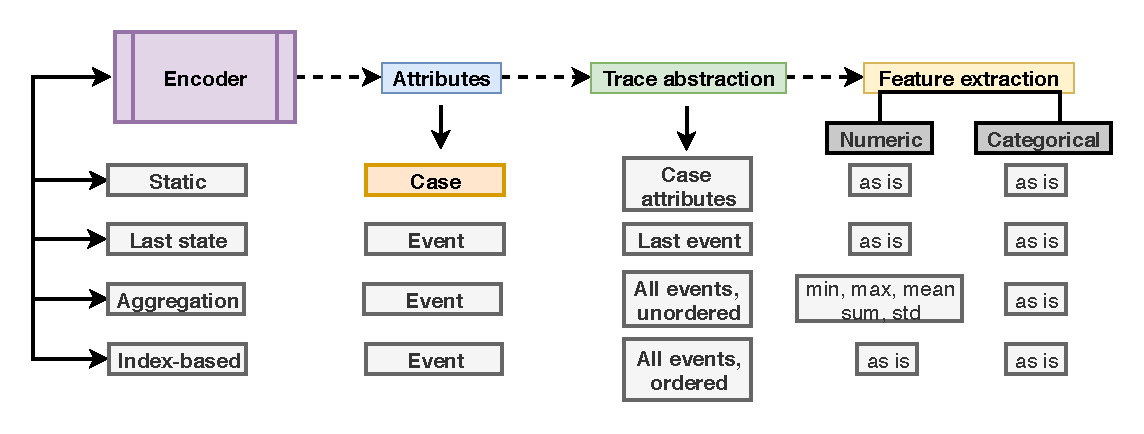
\includegraphics{images/general/cat_enc.pdf}}
		\caption{CatBoost with sequence encoding.}
		\label{fig:cat_enc}
	\end{center}
\end{figure}

 


\section{Complex Sequence Encoding} \label{dwt}
Each case in the event log carries information about events that describe its \textit{control flow} and each event is accompanied by information that describes the \textit{data flow}. Most of the existing sequence encoding methods consider only the control flow variables (i.e. simple sequence encoding) from each trace, and therefore it loses \textit{(lossy encoding)} information from historical event logs. In this thesis, we introduce a new complex sequence encoding approach.  This method is a \textit{lossless encoding} that captures information about control and data flow attributes with the help of \textit{discrete wavelet transformation and auto-encoder neural networks} (see figure \ref{fig:dwt1}).

\begin{figure}[htb]
	\begin{center}
		\resizebox{10cm}{!}{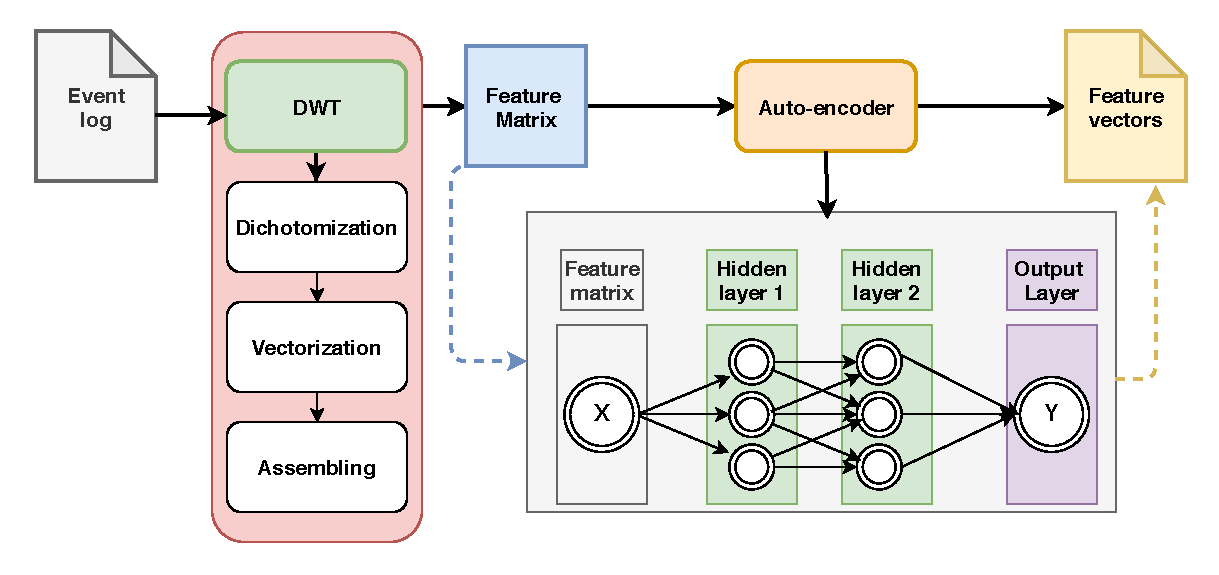
\includegraphics{images/general/dwt1.pdf}}
		\caption[Wavelet complex Sequence encoding]{Our approach to build a new complex sequence encoding method based on discrete wavelet transformation (DWT) and autoencoder neural network.}
		\label{fig:dwt1}
	\end{center}
\end{figure}


\subsection{Lossless encoding using Discrete Wavelet Transformation.}

In this section, we present a complex sequence encoding technique on the basis of \textit{discrete wavelet transformation} \cite{weeks2003discrete}, which is considered as a \textit{lossless} encoding method \cite{taymouri2019business}. In this approach, we encode each trace $\sigma$ in the event log $E$ into a group of vectors $V$ with an identical length for each event in the trace. Each vector includes the corresponding \textit{wavelet coefficients} for a distinct event. The significant perception is that for a given sequence of data, the \textit{wavelet coefficients} expose accessible varieties within this sequence at distinctive analyses \cite{taymouri2019business}.  Principally, each event log is composed of a collection of traces, and every trace contains many events, and each event has a specific timestamp associated with it, then wavelet coefficient is used to encode every timestamp in the event log. Formally, $\forall \sigma \in R, \sigma = \{e_1, e_2. \dots, e_k\}$ then $DWT(\sigma) = <v_1, v_2, \dots, v_k>$, where $|v_1| = |v_2| = \dots = |v_k|$. This method was first introduced in process mining to find the variance between two event logs \cite{taymouri2019business}.


For any \textit{vector space}, there is a tremendous amount of \textit{basis matrices} as a specific matrix can be acquired using the help of others by a linear transformation \cite{strang1993introduction}, for example, \textit{Haar transform matrix} which plays a significant role in analyzing time series (or sequential) data \cite{santoso1997power} such as event logs.

\newcommand{\tens}[1]{%
	\mathbin{\mathop{\otimes}\limits_{#1}}%
}

\begin{definition}{\textit{\textbf{Haar transform matrix}}}
	A Haar transform matrix is explained using the following recurrence equation as illustrated in \cite{rao1976orthogonal} for a dimension of $2^n$. 
	
	%A Haar basis matrix for a dimensional of power of two (i.e. %$2^n$) is explained using the following recurrence equation as %illustrated in 
	
	\begin{equation} \label{eq3}
	\begin{split}
	\textbf{T}(n) & = (\textbf{T}(n-1) \tens{} \begin{pmatrix}
	1  \\
	1
	\end{pmatrix}, \textbf{U}(n-1) \tens{} \begin{pmatrix}
	1  \\
	-1
	\end{pmatrix}, \textbf{T}(0)=1
	\end{split}
	\end{equation}
Where $\textbf{T}(n)$ is the \textit{Haar transform} that contains a set of vectors of length $2^n$, $\textit{U}(n)$ is a unit matrix  and $\tens{}$ is the outer product operator. For example: 

\begin{center}
	$\textbf{T}(1) = \begin{pmatrix}
	1 & 1  \\
	1 & -1
	\end{pmatrix}$
	,  and 
	$\textbf{T}(2) = \begin{pmatrix}
	1 & 1 & 1 & 0 \\
	1 & 1 & -1 & 0 \\
	1 & -1 & 0 & 1 \\
	1 & -1 & 0 & -1 

	\end{pmatrix}$
\end{center}	
	
\end{definition}


\begin{definition}{\textit{\textbf{Sequential data}}}
	A Sequential data $(s_1, \dots, s_j)$ is a sequence of data points ordered in time that is assumed to be real values taken at discrete intervals in time, e.g. from time $t=1$ to $time=j$ as defined in \cite{shumway2017time}.

\end{definition} 

\begin{definition}{\textit{\textbf{Discrete wavelet transformation}}}
	Discrete wavelet transformation $(DWT)$ is the representation of time series with \textit{Haar matrix} and \textit{wavelet coefficient}. 
		\begin{equation} \label{eq4}
	\begin{split}
	\textbf{DWT}(s) & = \textbf{T} \cdot \textbf{c}
	\end{split}
	\end{equation}
	
	Where $\textbf{T}$ is the Haar transform, and $\textbf{c}$ is a column vector that contains the \textit{wavelet coefficient}.	
\end{definition}
 
\begin{figure}[htb]
	\begin{center}
		\resizebox{10cm}{!}{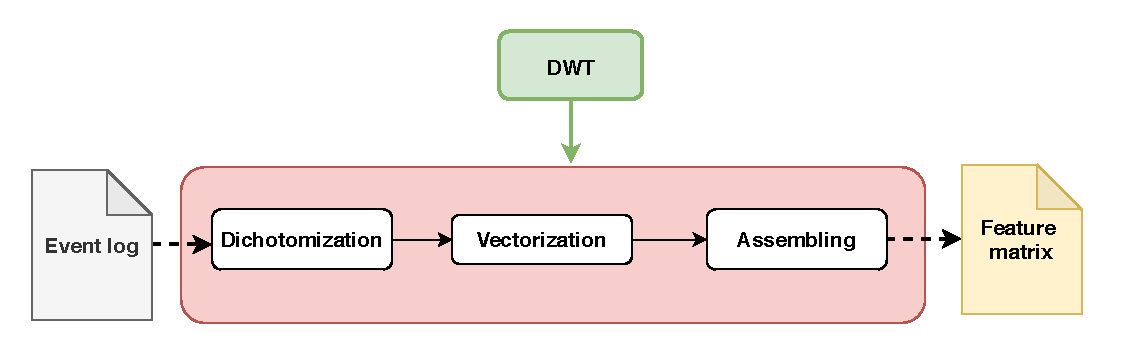
\includegraphics{images/general/dwt4.pdf}}
		\caption[Discrete wavelet transformation (DWT)]{Discrete wavelet transformation (WDT) takes an event log as input and encodes it to a feature vector by doing three main steps, i.e. dichotomization, vectorization, and assembling.}
		\label{fig:dwt4}
	\end{center}
\end{figure}

\subsection{DWT and autoencoder Neural network}
Complex sequence encoding using $DWT$ maps a trace into a multidimensional vector space. For each trace $\sigma$ in an event log $E$, it generates sets of multidimensional features. This approach has many advantages over other sequence encoding methods (see Chapter \ref{ch3}) such as: (\romannumeral 1) It is a lossless encoding method. (\romannumeral 2) Generated features are often uncorrelated \cite{aggarwal2015data, bakshi1999multiscale}. Subsequently working with a wavelet coefficient is the same as working with raw data without any loss of information. 

To encode event log using this approach into a feature vector we do three steps (see figure \ref{fig:dwt4}) for each trace: (\romannumeral 1) \textit{Dichotomization} which means extracting time series from a trace in the form of $\{0, 1\}$. $Zero$ when event $e$ does not exist in the input trace and $one$ if it exists; (\romannumeral 2) \textit{Vectorization} that encodes each time series into a vector through $DWT$ which is discrete in time and scale, meaning it catches together frequency and location in time information \cite{weeks2003discrete}; (\romannumeral 3) \textit{Assembling} combine all generated vectors that capture wavelet coefficient information into one single vector for each trace.  

\begin{definition}{\textit{\textbf{dichotomization}}}
 Let $\beta$ be all possible events or actions in an event log $E$ , and trace $\sigma$. we define function $B: \sigma \to  |\beta|$  to map each input trace in $E$ to a collection of $|\beta|$ sequential data of length $|\sigma|$. For example, $\sigma = <e_1, e_1, e_2, e_2>$ with $\beta = \{e_1, e_2, e_3\}$, then $B(e_1, \sigma) =1100$, and $B(e_2, \sigma) = 0011$, and $B(e_3, \sigma) = 0000$.	
\end{definition}


\begin{definition}{\textit{\textbf{Vectorization}}} \label{vect}
 we define function $V: B \to c$, that maps all time series into the relative \textit{wavelet coefficients}  where $B_i \in \{0,1\}$.Formally, $c = T^{-1} \cdot B$, where $T^{-1}$ is the inverse of Haar transform. Such as:
 
 \begin{center}
 	$\textbf{c}^{(i)} = \textbf{T}^{-1} \cdot s^{(i)}$\\
 	\vline
 	
 	$\textbf{c}^{(1)} = \begin{pmatrix}
 	0.25 & 0.25 & 0.25 & 0.25 \\
 	0.25 & 0.25 & -0.25 & -0.25 \\
 	0.5 & -0.5 & 0 & 0 \\
 	0 & 0 & 0.5 & -0.5  	
 	\end{pmatrix}$ $\cdot  \begin{pmatrix}
 		1 \\
 		1 \\
 		0 \\
 		0  	
 	\end{pmatrix}$\\
 	\vline\\
 	\vline
 	
 	$\textbf{c}^{(1)}=
 	\begin{pmatrix}
 		0.5 \\
 		0.5 \\
 		0 \\
 		0  	
 	\end{pmatrix}$, $\textbf{c}^{(1)}=
 \begin{pmatrix}
 0.5 \\
 -0.5 \\
 0 \\
 0  	
\end{pmatrix}$, $\textbf{c}^{(1)}=
\begin{pmatrix}
0 \\
0 \\
0 \\
0  	
\end{pmatrix} $

 \end{center}

\end{definition}


\begin{definition}{\textit{\textbf{Assembling}}} \label{ass}
	 We define $W$, i.e. a single vector for each trace $\sigma$ by combining all vectors from definition \ref{vect} into one vector such as $W(\sigma) = (c^{(1)}, \dots , c^{(n)}).$ For example:	
	 \begin{center}
	 	$W(\sigma) = <0.5, 0.5, 0, 0, 0.5, -0.5, 0, 0, 0, 0, 0, 0 >$
	 \end{center}
	 
\end{definition}

\begin{definition}{\textit{\textbf{Feature vector matrix}}}
 	Following the above definitions, we define a feature matrix $M$ for each event log $E$, which rows belong to the assembled vectors of the relative traces from definition \ref{ass}. 	
 	\begin{center}
 		$M(E) = \begin{pmatrix}
 		W(\sigma_1) \\
 		\vdots\\
 		W(\sigma_n)
 		\end{pmatrix} $
 	\end{center}
\end{definition}
 
Following the above definitions, we built a new complex sequence encoding method based on discrete wavelet transformation and time-series encoding by mapping each event log into a feature vector matrix whose rows are related to wavelet coefficients for each trace in the event log. This encoding method has two drawbacks compared to other encoding methods (see Chapter \ref{ch3}): (\romannumeral 1) The time complexity in the worst case is $O(n^3)$ w.r.t the largest business case in the event log. Accordingly, for large datasets, this encoding method takes much time just to encode historical events into a numerical feature vector; (\romannumeral 2) secondly, is the generated feature matrix is a \textit{highly sparse multidimensional matrix}. To overcome this drawback, we can select a subset from the feature matrix based on the importance or apply one of the dimension reduction techniques.  We decided to use an \textit{auto-encoder} neural network to reduce the dimensionality of the feature matrix and to retain all information of the historical event logs. 

\textit{Auto-encoder} is an unsupervised method that tries to remove noise or unnecessary information from the original data. The idea of a neural network encoder is to compress the information that exists in the feature matrix with high dimensional space into a low dimensional space.  After encoding each trace in the original event log using $DWT$, we pass it to the auto-encoder method (see figure \ref{fig:dwt1}) that compresses it into a lower dimension. 


Following the general work-flow of outcome-oriented predictive process monitoring in Chapter \ref{ch3} section \ref{wf}, we changed \textit{sequence encoding} methods to add our proposed complex sequence encoding method using \textit{$DWT$, and auto-encoders} Figure \ref{fig:dwt5} shows the changes to all encoding methods w.r.t Sequence encoding.

\begin{figure}[htb]
	\begin{center}
		\resizebox{10cm}{!}{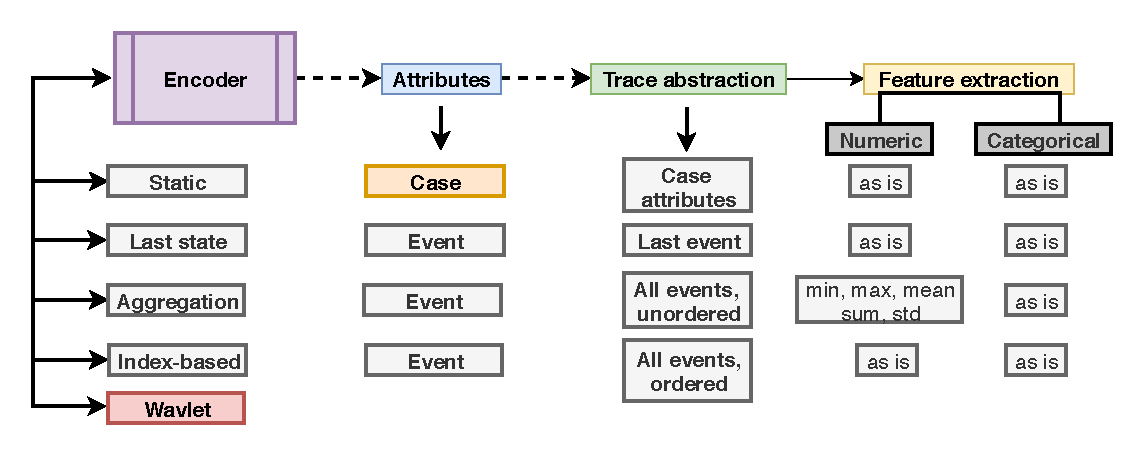
\includegraphics{images/general/dwt5.pdf}}
		\caption[Wavelet encoding method taxonomy]{Taxonomy of existing and proposed (i.e. wavelet) sequence encoding methods for outcome-oriented PPM.}
		\label{fig:dwt5}
	\end{center}
\end{figure}

\section{Inter-case features} \label{inter}
In recent predictive process monitoring methods, the outcome mainly comes from the execution of the current running business process (i.e. \textit{intra-case features}), on the other hand, in real-life systems the outcome does not depend only on the running case, but it depends on features that come from the concurrent execution of all business cases (i.e. \textit{inter-case features}). For example, in many scenarios ongoing cases compete with each other for resources, then the number of ongoing cases that share the same resource  may be a bottleneck to predict the outcome for an incomplete business case. In this section, we introduce new inter-case features that improve the outcome-oriented PPM in w.r.t the prediction accuracy.

In \cite{senderovich2019knowledge} they introduced a two-dimensional method for feature encoding, where the first dimension depends on the intra-case features, and the second one relies on the inter-case features. For the inter-case dimension, they proposed two different approaches: (\romannumeral 1) \textit{A knowledge-driven encoding (KDE)}, that relies on the previous knowledge about cases; (\romannumeral 2) \textit{A data-driven encoding (DDE)}, that defines cases automatically from event logs employing proximity metrics. 

In this thesis, we propose three different categories of inter-case features (see figure \ref{fig:inter1}): (\romannumeral 1) \textit{Workload} features; (\romannumeral 2) \textit{Demand intensity} features; (\romannumeral 3) \textit{Temporal contextual} features with an experimental evaluation executed on 20 event logs.

\begin{figure}[htb]
	\begin{center}
		\resizebox{10cm}{!}{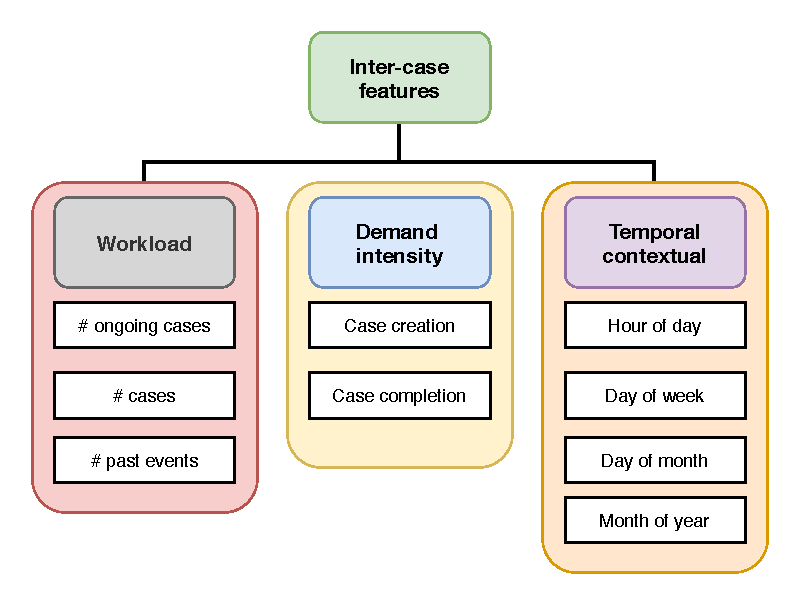
\includegraphics{images/general/inter1.pdf}}
		\caption[Inter-case features]{Categorization of inter-case features that we propose in this thesis, i.e. workload, demand intensity, and temporal contextual features.
		}
		\label{fig:inter1}
	\end{center}
\end{figure}

\textit{Workload features.} To improve the overall performance of business processes, we need to maximize the utilization of resources that we have in our system. Accordingly, monitoring and managing workload is crucial to any business process. In this context, we define three different inter-case features that capture information about the workload. (\romannumeral 1) The number of business cases that have started and not finished; (\romannumeral 2) The number of activities that happened in the last $x$ minutes or hour; (\romannumeral 3) Let $C$ be an ongoing case, and  $e_c$ be the last event observed in $C$  we define an inter-case feature that captures information about the number of other ongoing cases where the last event is $e_c$.

\textit{Demand intensity.} The purpose of demand intensity analysis is demand prediction, and therefore, in terms of determining a proper resource to work on a specific action or activity, we need to monitor the intensity of business process creation and completion.   to address this point, we define tow different features that capture information about the request intensity. (\romannumeral 1) \textit{Case creation intensity} that carries information about How many new cases were created since the current case started (divided by the number of seconds since the current case was created). (\romannumeral 2) \textit{Case completion intensity} on the other hand capture information about how many cases have completed since this case was created divided by the number of seconds since the current case was created.


\textit{Temporal contextual} Temporal information extraction has grown in the area of outcome-oriented PPM, and it is meant to capture circadian cycles, i.e. current time's hour of the day $(0-23)$, and day of the week when the last event in the current case occurred $(1-7)$. In this context, we defined four different inter-case features: (\romannumeral 1) Hour of the day; (\romannumeral 2) Day of the week; (\romannumeral 3) Day of the month; (\romannumeral 4) Month of the year; 



\section{Summary}
This Chapter answer RQ4 by giving a complete description of our three different proposed approaches to improve the outcome-oriented predictive process monitoring tasks. In the next Chapter, we start by setting experiments to evaluate proposed methods in comparison to currently existing techniques. 



% ---------------------------------------------------------------------------
%: ----------------------- end of thesis sub-document ------------------------
% ---------------------------------------------------------------------------

